% Created by tikzDevice version 0.10.1 on 2017-10-12 17:15:21
% !TEX encoding = UTF-8 Unicode
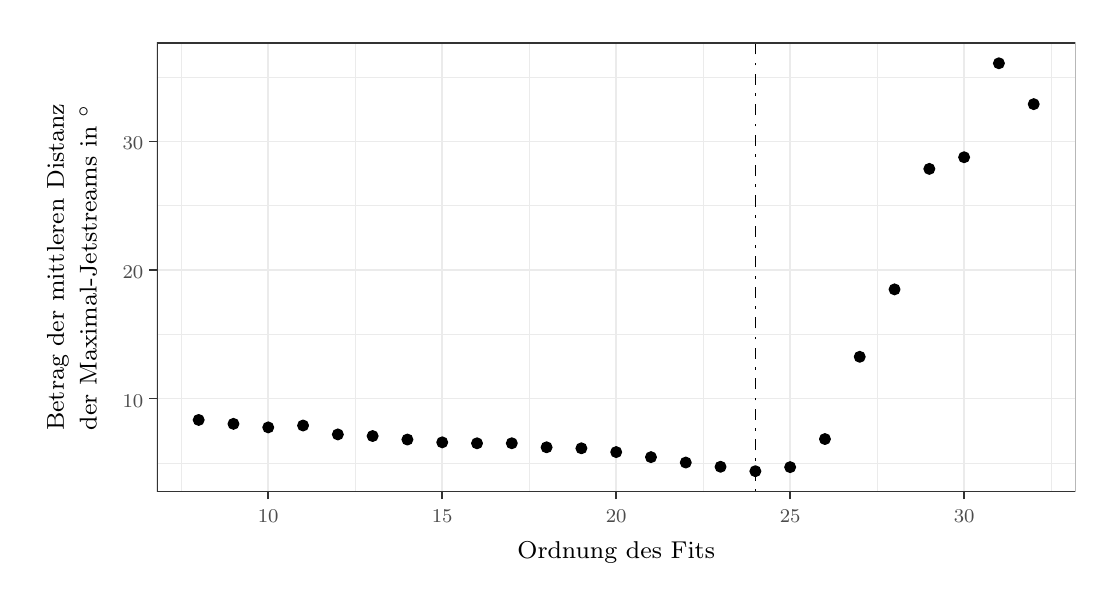
\begin{tikzpicture}[font=\footnotesize,x=1pt,y=1pt]
\definecolor{fillColor}{RGB}{255,255,255}
\path[use as bounding box,fill=fillColor,fill opacity=0.00] (0,0) rectangle (384.11,199.17);
\begin{scope}
\path[clip] (  0.00,  0.00) rectangle (384.11,199.17);
\definecolor{drawColor}{RGB}{255,255,255}
\definecolor{fillColor}{RGB}{255,255,255}

\path[draw=drawColor,line width= 0.6pt,line join=round,line cap=round,fill=fillColor] (  0.00,  0.00) rectangle (384.11,199.17);
\end{scope}
\begin{scope}
\path[clip] ( 46.70, 31.53) rectangle (378.61,193.67);
\definecolor{fillColor}{RGB}{255,255,255}

\path[fill=fillColor] ( 46.70, 31.53) rectangle (378.61,193.67);
\definecolor{drawColor}{gray}{0.92}

\path[draw=drawColor,line width= 0.3pt,line join=round] ( 46.70, 41.89) --
	(378.61, 41.89);

\path[draw=drawColor,line width= 0.3pt,line join=round] ( 46.70, 88.33) --
	(378.61, 88.33);

\path[draw=drawColor,line width= 0.3pt,line join=round] ( 46.70,134.78) --
	(378.61,134.78);

\path[draw=drawColor,line width= 0.3pt,line join=round] ( 46.70,181.23) --
	(378.61,181.23);

\path[draw=drawColor,line width= 0.3pt,line join=round] ( 55.50, 31.53) --
	( 55.50,193.67);

\path[draw=drawColor,line width= 0.3pt,line join=round] (118.37, 31.53) --
	(118.37,193.67);

\path[draw=drawColor,line width= 0.3pt,line join=round] (181.23, 31.53) --
	(181.23,193.67);

\path[draw=drawColor,line width= 0.3pt,line join=round] (244.09, 31.53) --
	(244.09,193.67);

\path[draw=drawColor,line width= 0.3pt,line join=round] (306.95, 31.53) --
	(306.95,193.67);

\path[draw=drawColor,line width= 0.3pt,line join=round] (369.81, 31.53) --
	(369.81,193.67);

\path[draw=drawColor,line width= 0.6pt,line join=round] ( 46.70, 65.11) --
	(378.61, 65.11);

\path[draw=drawColor,line width= 0.6pt,line join=round] ( 46.70,111.56) --
	(378.61,111.56);

\path[draw=drawColor,line width= 0.6pt,line join=round] ( 46.70,158.00) --
	(378.61,158.00);

\path[draw=drawColor,line width= 0.6pt,line join=round] ( 86.93, 31.53) --
	( 86.93,193.67);

\path[draw=drawColor,line width= 0.6pt,line join=round] (149.80, 31.53) --
	(149.80,193.67);

\path[draw=drawColor,line width= 0.6pt,line join=round] (212.66, 31.53) --
	(212.66,193.67);

\path[draw=drawColor,line width= 0.6pt,line join=round] (275.52, 31.53) --
	(275.52,193.67);

\path[draw=drawColor,line width= 0.6pt,line join=round] (338.38, 31.53) --
	(338.38,193.67);
\definecolor{drawColor}{RGB}{0,0,0}
\definecolor{fillColor}{RGB}{0,0,0}

\path[draw=drawColor,line width= 0.4pt,line join=round,line cap=round,fill=fillColor] ( 61.79, 57.42) circle (  1.96);

\path[draw=drawColor,line width= 0.4pt,line join=round,line cap=round,fill=fillColor] ( 74.36, 56.01) circle (  1.96);

\path[draw=drawColor,line width= 0.4pt,line join=round,line cap=round,fill=fillColor] ( 86.93, 54.73) circle (  1.96);

\path[draw=drawColor,line width= 0.4pt,line join=round,line cap=round,fill=fillColor] ( 99.51, 55.41) circle (  1.96);

\path[draw=drawColor,line width= 0.4pt,line join=round,line cap=round,fill=fillColor] (112.08, 52.19) circle (  1.96);

\path[draw=drawColor,line width= 0.4pt,line join=round,line cap=round,fill=fillColor] (124.65, 51.61) circle (  1.96);

\path[draw=drawColor,line width= 0.4pt,line join=round,line cap=round,fill=fillColor] (137.22, 50.34) circle (  1.96);

\path[draw=drawColor,line width= 0.4pt,line join=round,line cap=round,fill=fillColor] (149.80, 49.33) circle (  1.96);

\path[draw=drawColor,line width= 0.4pt,line join=round,line cap=round,fill=fillColor] (162.37, 48.98) circle (  1.96);

\path[draw=drawColor,line width= 0.4pt,line join=round,line cap=round,fill=fillColor] (174.94, 49.00) circle (  1.96);

\path[draw=drawColor,line width= 0.4pt,line join=round,line cap=round,fill=fillColor] (187.51, 47.54) circle (  1.96);

\path[draw=drawColor,line width= 0.4pt,line join=round,line cap=round,fill=fillColor] (200.09, 47.18) circle (  1.96);

\path[draw=drawColor,line width= 0.4pt,line join=round,line cap=round,fill=fillColor] (212.66, 45.81) circle (  1.96);

\path[draw=drawColor,line width= 0.4pt,line join=round,line cap=round,fill=fillColor] (225.23, 43.98) circle (  1.96);

\path[draw=drawColor,line width= 0.4pt,line join=round,line cap=round,fill=fillColor] (237.80, 42.03) circle (  1.96);

\path[draw=drawColor,line width= 0.4pt,line join=round,line cap=round,fill=fillColor] (250.37, 40.50) circle (  1.96);

\path[draw=drawColor,line width= 0.4pt,line join=round,line cap=round,fill=fillColor] (262.95, 38.90) circle (  1.96);

\path[draw=drawColor,line width= 0.4pt,line join=round,line cap=round,fill=fillColor] (275.52, 40.37) circle (  1.96);

\path[draw=drawColor,line width= 0.4pt,line join=round,line cap=round,fill=fillColor] (288.09, 50.52) circle (  1.96);

\path[draw=drawColor,line width= 0.4pt,line join=round,line cap=round,fill=fillColor] (300.66, 80.24) circle (  1.96);

\path[draw=drawColor,line width= 0.4pt,line join=round,line cap=round,fill=fillColor] (313.24,104.60) circle (  1.96);

\path[draw=drawColor,line width= 0.4pt,line join=round,line cap=round,fill=fillColor] (325.81,148.14) circle (  1.96);

\path[draw=drawColor,line width= 0.4pt,line join=round,line cap=round,fill=fillColor] (338.38,152.35) circle (  1.96);

\path[draw=drawColor,line width= 0.4pt,line join=round,line cap=round,fill=fillColor] (350.95,186.30) circle (  1.96);

\path[draw=drawColor,line width= 0.4pt,line join=round,line cap=round,fill=fillColor] (363.53,171.54) circle (  1.96);

\path[draw=drawColor,line width= 0.6pt,dash pattern=on 1pt off 3pt on 4pt off 3pt ,line join=round] (262.95, 31.53) -- (262.95,193.67);
\definecolor{drawColor}{gray}{0.20}

\path[draw=drawColor,line width= 0.6pt,line join=round,line cap=round] ( 46.70, 31.53) rectangle (378.61,193.67);
\end{scope}
\begin{scope}
\path[clip] (  0.00,  0.00) rectangle (384.11,199.17);
\definecolor{drawColor}{gray}{0.30}

\node[text=drawColor,anchor=base east,inner sep=0pt, outer sep=0pt, scale=  0.88] at ( 41.75, 62.08) {10};

\node[text=drawColor,anchor=base east,inner sep=0pt, outer sep=0pt, scale=  0.88] at ( 41.75,108.53) {20};

\node[text=drawColor,anchor=base east,inner sep=0pt, outer sep=0pt, scale=  0.88] at ( 41.75,154.97) {30};
\end{scope}
\begin{scope}
\path[clip] (  0.00,  0.00) rectangle (384.11,199.17);
\definecolor{drawColor}{gray}{0.20}

\path[draw=drawColor,line width= 0.6pt,line join=round] ( 43.95, 65.11) --
	( 46.70, 65.11);

\path[draw=drawColor,line width= 0.6pt,line join=round] ( 43.95,111.56) --
	( 46.70,111.56);

\path[draw=drawColor,line width= 0.6pt,line join=round] ( 43.95,158.00) --
	( 46.70,158.00);
\end{scope}
\begin{scope}
\path[clip] (  0.00,  0.00) rectangle (384.11,199.17);
\definecolor{drawColor}{gray}{0.20}

\path[draw=drawColor,line width= 0.6pt,line join=round] ( 86.93, 28.78) --
	( 86.93, 31.53);

\path[draw=drawColor,line width= 0.6pt,line join=round] (149.80, 28.78) --
	(149.80, 31.53);

\path[draw=drawColor,line width= 0.6pt,line join=round] (212.66, 28.78) --
	(212.66, 31.53);

\path[draw=drawColor,line width= 0.6pt,line join=round] (275.52, 28.78) --
	(275.52, 31.53);

\path[draw=drawColor,line width= 0.6pt,line join=round] (338.38, 28.78) --
	(338.38, 31.53);
\end{scope}
\begin{scope}
\path[clip] (  0.00,  0.00) rectangle (384.11,199.17);
\definecolor{drawColor}{gray}{0.30}

\node[text=drawColor,anchor=base,inner sep=0pt, outer sep=0pt, scale=  0.88] at ( 86.93, 20.52) {10};

\node[text=drawColor,anchor=base,inner sep=0pt, outer sep=0pt, scale=  0.88] at (149.80, 20.52) {15};

\node[text=drawColor,anchor=base,inner sep=0pt, outer sep=0pt, scale=  0.88] at (212.66, 20.52) {20};

\node[text=drawColor,anchor=base,inner sep=0pt, outer sep=0pt, scale=  0.88] at (275.52, 20.52) {25};

\node[text=drawColor,anchor=base,inner sep=0pt, outer sep=0pt, scale=  0.88] at (338.38, 20.52) {30};
\end{scope}
\begin{scope}
\path[clip] (  0.00,  0.00) rectangle (384.11,199.17);
\definecolor{drawColor}{RGB}{0,0,0}

\node[text=drawColor,anchor=base,inner sep=0pt, outer sep=0pt, scale=  1.10] at (212.66,  7.44) {Ordnung des Fits};
\end{scope}
\begin{scope}
\path[clip] (  0.00,  0.00) rectangle (384.11,199.17);
\definecolor{drawColor}{RGB}{0,0,0}

\node[text=drawColor,rotate= 90.00,anchor=base,inner sep=0pt, outer sep=0pt, scale=  1.10] at ( 13.08,112.60) {Betrag der mittleren Distanz };

\node[text=drawColor,rotate= 90.00,anchor=base,inner sep=0pt, outer sep=0pt, scale=  1.10] at ( 24.96,112.60) { der Maximal-Jetstreams in $^{\circ}$};
\end{scope}
\end{tikzpicture}
